% Provenance (never printed): cycle 4 SVT/physique, "La planete Terre,
% l'environnement": the movements of the atmosphere, weather and its
% forecast; see sources/book1/PROVENANCE.md. Book 1, grade 8, chapter 3.
% Vocabulary guard: owns air mass, front (warm, cold), depression (homograph:
% phrase-level linking only), anticyclone, isobar, weather forecast. The
% rotation of the winds around lows and highs is told (deflection, recalled
% from ch. g8.2); the occluded front is named in prose only; numerical models
% are told, not taught.
\chapter{Masses d'air, fronts et cartes météorologiques}\label{ch:g8:fronts-and-weather-maps}

Le matin est clair et calme. Vers midi, de fines traînées blanches
apparaissent très haut dans le ciel, puis s'étalent lentement en un voile
pâle qui ternit le Soleil. L'après-midi, les \omterm{def:g4:clouds-rain-snow:cloud}{nuages} s'épaississent et
descendent~; le soir, une \omterm{def:g4:clouds-rain-snow:precipitation}{pluie} continue tombe. Pendant la nuit, l'air
devient doux et humide, puis une ligne sombre de \omterm{def:g4:clouds-rain-snow:cloud}{nuages} apporte une courte
averse violente et un coup de vent. Le lendemain matin est clair, frais et
venté. En deux jours, une \emph{\omterm{def:g8:fronts-and-weather-maps:depression}{dépression}} est passée sur la ville, avec
ses deux \omterm{def:g8:fronts-and-weather-maps:front}{fronts}.
% ledger: ucar:warm-front, ucar:cold-front

\begin{omfigure}
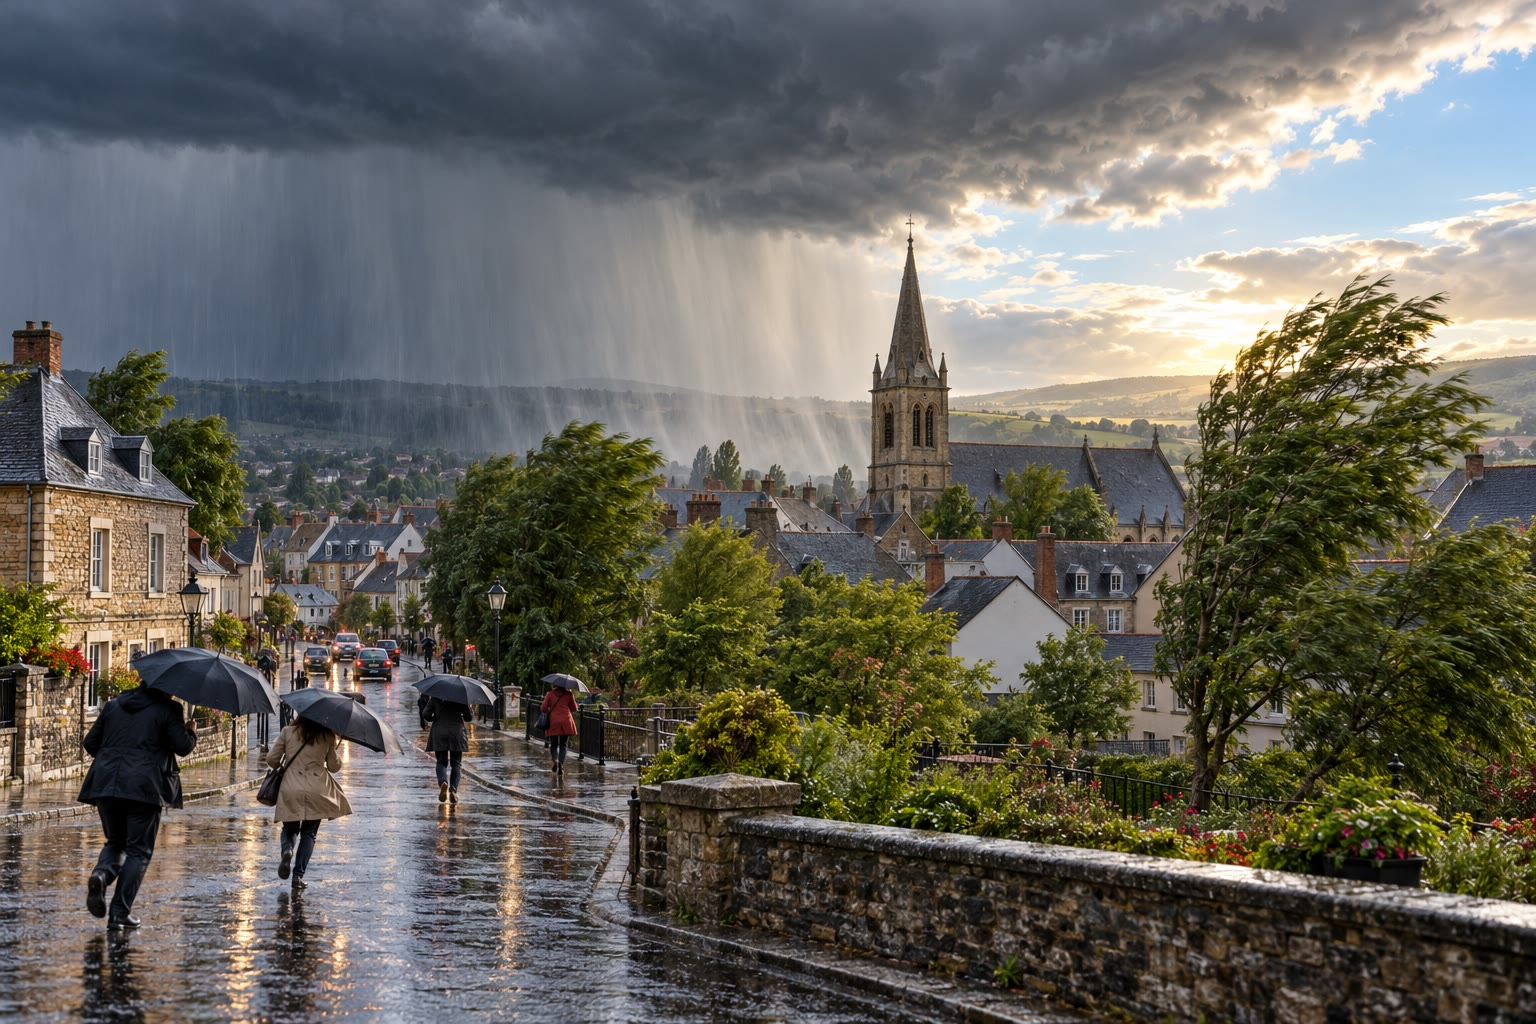
\includegraphics[width=0.6\linewidth]{images/book1/ai/g8-rain-arriving.jpg}

{\small Un rideau de \omterm{def:g4:clouds-rain-snow:precipitation}{pluie} arrive sur une ville sous une base de \omterm{def:g4:clouds-rain-snow:cloud}{nuages}
sombre, alors que le ciel est encore clair derrière l'église (illustration
générée par IA d'une scène générique).}
\label{fig:g8:fronts-and-weather-maps:rain}
\end{omfigure}

Les prévisionnistes l'avaient vue venir plusieurs jours à l'avance. Ce
chapitre montre comment~: l'air de notre ciel arrive en grandes masses,
les masses se rencontrent le long de \omterm{def:g8:fronts-and-weather-maps:front}{fronts}, et les \omterm{def:g2:drawing-to-map:map}{cartes} de la pression
montrent où elles vont.

\begin{recall}
L'air appuie sur tout ce qu'il touche~; un baromètre mesure cette pression
en hectopascals (les livres de physique), et au \omterm{def:g4:world-physical-map:altitude}{niveau de la mer} elle vaut
environ \qty{1013}{hPa} (\cref{ch:g8:the-atmosphere}). Les \omterm{def:g4:clouds-rain-snow:cloud}{nuages} se
forment quand de l'air humide monte et se refroidit
(\cref{ch:g4:clouds-rain-snow}). Au sol, le vent souffle des hautes
pressions vers les basses pressions, et la rotation de la Terre le
dévie~: vers la droite dans l'\omterm{def:g3:continents-and-oceans:equator}{hémisphère} Nord. Entre environ \ang{30} et
\ang{60}, les \omterm{def:g8:winds-global-circulation:global-winds}{vents d'ouest} amènent une \omterm{def:g5:natural-hazards:storm}{tempête} après l'autre
(\cref{ch:g8:winds-global-circulation}).
\end{recall}

\section{Les masses d'air}

L'air qui reste plusieurs jours au-dessus du même endroit prend le
caractère de la surface qui se trouve au-dessous. Au-dessus d'un \omterm{def:g2:water-on-earth:ocean}{océan}
chaud, il devient chaud et humide~; au-dessus d'une terre gelée, froid et
sec. Quand il s'en va, il emporte ce caractère avec lui, parfois sur des
milliers de kilomètres.
% ledger: noaa:air-mass

\begin{definition}[Masse d'air]\label{def:g8:fronts-and-weather-maps:air-mass}
Une \emph{masse d'air}\index{masse d'air} est un très grand volume d'air
dans lequel la température et l'humidité sont presque les mêmes partout à
une \omterm{def:g4:world-physical-map:altitude}{altitude} donnée. Elle les tient de la région où elle s'est formée, sa
\emph{région source}.
\end{definition}
% ledger: noaa:air-mass

Les prévisionnistes désignent une \omterm{def:g8:fronts-and-weather-maps:air-mass}{masse d'air} par deux lettres. La
première dit où elle s'est formée~: \emph{c} (continentale) au-dessus des
terres, elle est donc sèche~; \emph{m} (maritime) au-dessus d'un \omterm{def:g2:water-on-earth:ocean}{océan},
elle est donc humide. La seconde dit à quel point elle est froide~:
\emph{A} (arctique) au-dessus des régions polaires, \emph{P} (polaire)
au-dessus des hautes \omterm{def:g6:latitude-longitude:latitude}{latitudes}, \emph{T} (tropicale) au-dessus des basses
\omterm{def:g6:latitude-longitude:latitude}{latitudes}. L'air d'un \omterm{def:g5:weather-and-climate:desert}{désert} chaud est cT, chaud et sec~; l'air de
l'Arctique est cA, très froid et sec.
% ledger: noaa:air-mass

\begin{omfigure}
\begin{tikzpicture}
\begin{axis}[ommap, width=12.6cm, xmin=-100, xmax=60, ymin=10, ymax=85,
  xtick={-90,-60,...,60}, ytick={20,40,60,80},
  xticklabels={$90^\circ$O,$60^\circ$O,$30^\circ$O,$0^\circ$,$30^\circ$E,$60^\circ$E},
  yticklabels={$20^\circ$N,$40^\circ$N,$60^\circ$N,$80^\circ$N},
  tick label style={font=\scriptsize}]
  \addplot[fill=omLithAlluv, draw=black!45, line width=0.2pt] table {figdata/out/shared-geo-land.dat};
  \tikzset{src/.style={line width=0.9pt, fill opacity=0.35, text opacity=1, font=\scriptsize, align=center}}
  \draw[src, draw=omCold, fill=omCold!35] (axis cs:-30,79) ellipse [x radius=26, y radius=4.5];
  \node[font=\scriptsize, align=center, fill=white, inner sep=1pt] at (axis cs:-30,79) {\textbf{cA}~: très froide, sèche};
  \draw[src, draw=omCold, fill=omCold!25] (axis cs:-35,55) ellipse [x radius=14, y radius=6];
  \node[font=\scriptsize, align=center, fill=white, inner sep=1pt] at (axis cs:-35,55) {\textbf{mP}~: froide,\\ humide};
  \draw[src, draw=omCold, fill=omCold!25] (axis cs:-84,60) ellipse [x radius=12, y radius=7];
  \node[font=\scriptsize, align=center, fill=white, inner sep=1pt] at (axis cs:-84,60) {\textbf{cP}~: froide,\\ sèche};
  \draw[src, draw=omCold, fill=omCold!25] (axis cs:45,62) ellipse [x radius=14, y radius=7];
  \node[font=\scriptsize, align=center, fill=white, inner sep=1pt] at (axis cs:45,62) {\textbf{cP}~: froide,\\ sèche};
  \draw[src, draw=omWarm, fill=omWarm!25] (axis cs:-45,28) ellipse [x radius=16, y radius=6];
  \node[font=\scriptsize, align=center, fill=white, inner sep=1pt] at (axis cs:-45,28) {\textbf{mT}~: chaude,\\ humide};
  \draw[src, draw=omWarm, fill=omWarm!25] (axis cs:10,24) ellipse [x radius=15, y radius=6];
  \node[font=\scriptsize, align=center, fill=white, inner sep=1pt] at (axis cs:10,24) {\textbf{cT}~: très chaude,\\ sèche};
\end{axis}
\end{tikzpicture}

{\small Des régions sources typiques des \omterm{def:g8:fronts-and-weather-maps:air-mass}{masses d'air} autour de
l'Atlantique Nord (schéma)~: au-dessus de l'Arctique, des \omterm{def:g3:continents-and-oceans:continent}{continents}
froids, de l'\omterm{def:g2:water-on-earth:ocean}{océan} du Nord, de l'\omterm{def:g2:water-on-earth:ocean}{océan} subtropical et du Sahara. En bleu~:
les \omterm{def:g8:fronts-and-weather-maps:air-mass}{masses d'air} froides~; en rouge~: les chaudes.}
% ledger: noaa:air-mass, data:ne-land (schematic regions)
\label{fig:g8:fronts-and-weather-maps:sources}
\end{omfigure}

\section{Les fronts}

Quand une \omterm{def:g8:fronts-and-weather-maps:air-mass}{masse d'air} se déplace, elle en rencontre une autre. Les deux ne
se mélangent pas facilement~: elles restent séparées, avec entre elles une
étroite limite où le temps change.
% ledger: mo:fronts, ucar:cold-front

\begin{definition}[Front]\label{def:g8:fronts-and-weather-maps:front}
Un \emph{front}\index{front} est la limite, au sol, entre deux \omterm{def:g8:fronts-and-weather-maps:air-mass}{masses
d'air} de température et d'humidité différentes. À un \emph{front froid}\index{front froid},
l'air froid pousse l'air plus chaud et prend sa place~; à un
\emph{front chaud}\index{front chaud}, l'air chaud pousse l'air plus froid
et prend sa place.
\end{definition}
% ledger: mo:fronts, ucar:cold-front, ucar:warm-front

L'air froid est plus dense que l'air chaud. À un \omterm{def:g8:fronts-and-weather-maps:front}{front froid}, l'air froid
se glisse sous l'air chaud comme un coin et le soulève brusquement. L'air
chaud et humide monte vite et forme des \omterm{def:g4:clouds-rain-snow:cloud}{nuages} qui s'élèvent comme des
tours, \omterm{def:g4:clouds-rain-snow:cloud-families}{cumulus} et \omterm{def:g4:clouds-rain-snow:cloud-families}{cumulonimbus}~: le \omterm{def:g8:fronts-and-weather-maps:front}{front} apporte de fortes averses,
parfois de la \omterm{def:g4:clouds-rain-snow:precipitation}{grêle} et du tonnerre, des rafales de vent et une baisse
soudaine de la température. Une fois qu'il est passé, la \omterm{def:g4:clouds-rain-snow:precipitation}{pluie} cesse et le
ciel se dégage. Un \omterm{def:g8:fronts-and-weather-maps:front}{front froid} avance vite, jusqu'à deux fois plus vite
qu'un \omterm{def:g8:fronts-and-weather-maps:front}{front chaud}.
% ledger: ucar:cold-front

\begin{omfigure}
\begin{tikzpicture}[font=\footnotesize, >={Stealth[length=2.2mm]}, yscale=0.7, xscale=0.95]
  % ground
  \draw[line width=0.8pt] (0,0) -- (15,0);
  % cold wedge, nose at x = 8.2
  \fill[omCold!18] (0,0) -- (0,3.4) .. controls (4.5,3.2) and (7.2,2.4) .. (7.9,0.8)
    .. controls (8.1,0.35) and (8.2,0.12) .. (8.25,0) -- cycle;
  \draw[omCold, line width=1pt] (0,3.4) .. controls (4.5,3.2) and (7.2,2.4) .. (7.9,0.8)
    .. controls (8.1,0.35) and (8.2,0.12) .. (8.25,0);
  \node[omCold, align=center] at (3.2,1.4) {\textbf{air froid}\\(dense)};
  \node[omWarm, align=center] at (12.6,1.4) {\textbf{air chaud et humide}};
  % cold air pushes
  \draw[->, omCold, line width=1.2pt] (4.6,0.5) -- (7.0,0.5);
  % warm air lifted
  \draw[->, omWarm, line width=1.2pt] (11.2,0.45) .. controls (9.4,0.6) and (8.6,1.4) .. (8.5,3.0);
  % cumulonimbus
  \fill[black!12] (7.3,2.6) .. controls (7.0,3.4) and (7.4,4.2) .. (7.9,4.5)
    .. controls (7.6,5.0) and (8.6,5.2) .. (9.4,5.1) -- (11.0,5.15)
    .. controls (10.6,4.9) and (10.2,4.8) .. (10.0,4.6)
    .. controls (10.4,4.0) and (10.2,3.0) .. (9.8,2.5) -- cycle;
  \draw[black!45] (7.3,2.6) .. controls (7.0,3.4) and (7.4,4.2) .. (7.9,4.5)
    .. controls (7.6,5.0) and (8.6,5.2) .. (9.4,5.1) -- (11.0,5.15)
    .. controls (10.6,4.9) and (10.2,4.8) .. (10.0,4.6)
    .. controls (10.4,4.0) and (10.2,3.0) .. (9.8,2.5) -- cycle;
  \node at (9.0,3.8) {cumulonimbus};
  \foreach \x in {7.7,8.0,...,9.6} \draw[omCold!70, line width=0.5pt] (\x,2.45) -- (\x-0.25,0.15);
  \node[anchor=west, align=left] at (9.8,1.95) {fortes averses,\\rafales};
  % motion
  \draw[->, line width=1.3pt] (5.7,4.3) -- (7.2,4.3);
  \node[anchor=east] at (5.6,4.3) {le front avance};
  \node[anchor=north] at (8.25,-0.1) {front au sol};
  \node[anchor=north west, align=left] at (0.1,-0.1) {derrière~: plus frais, éclaircies};
  \node[anchor=north east, align=right] at (15,-0.1) {devant~: chaud et humide};
\end{tikzpicture}

{\small Un \omterm{def:g8:fronts-and-weather-maps:front}{front froid} vu de côté (hauteurs très exagérées). L'air froid
se glisse sous l'air chaud comme un coin~; l'air chaud est soulevé
brusquement et forme des \omterm{def:g4:clouds-rain-snow:cloud}{nuages} qui s'élèvent comme des tours.}
% ledger: ucar:cold-front
\label{fig:g8:fronts-and-weather-maps:cold}
\end{omfigure}

À un \omterm{def:g8:fronts-and-weather-maps:front}{front chaud}, l'air chaud, léger, ne peut pas chasser l'air froid du
sol~: il monte lentement par-dessus, sur une pente longue et douce. Ses
\omterm{def:g4:clouds-rain-snow:cloud}{nuages} apparaissent donc loin en avant du \omterm{def:g8:fronts-and-weather-maps:front}{front}, haut dans le ciel~:
d'abord de fines traînées de \omterm{def:g4:clouds-rain-snow:cloud-families}{cirrus}, puis un voile de cirrostratus, puis
des altostratus gris. À mesure que le \omterm{def:g8:fronts-and-weather-maps:front}{front} approche, les \omterm{def:g4:clouds-rain-snow:cloud}{nuages}
descendent et s'épaississent, et une longue \omterm{def:g4:clouds-rain-snow:precipitation}{pluie} continue commence. Après
son passage, l'air est plus chaud et plus humide.
% ledger: ucar:warm-front, bom:isobars (warm front: steady rain, grey skies)

\begin{omfigure}
\begin{tikzpicture}[font=\footnotesize, >={Stealth[length=2.2mm]}]
  \draw[line width=0.8pt] (0,0) -- (15,0);
  % cold air ahead (right), warm air climbing a gentle slope from the front at x = 2.2
  \fill[omCold!18] (2.2,0) .. controls (6,0.9) and (10,2.2) .. (15,3.4) -- (15,0) -- cycle;
  \draw[omCold, line width=1pt] (2.2,0) .. controls (6,0.9) and (10,2.2) .. (15,3.4);
  \node[omCold, align=center] at (11.8,0.75) {\textbf{air froid}};
  \node[omWarm, align=center] at (1.4,1.6) {\textbf{air chaud}\\\textbf{et humide}};
  \draw[->, omWarm, line width=1.2pt] (1.0,0.45) .. controls (4.5,0.9) and (8.5,2.4) .. (12.4,3.4);
  % clouds: nimbostratus near the front, altostratus, cirrostratus, cirrus far ahead
  \fill[black!18] (2.4,0.7) .. controls (3.2,1.8) and (5.5,2.3) .. (6.6,2.4) -- (6.4,1.25) .. controls (5,1.0) and (3.8,0.7) .. cycle;
  \node at (5.4,1.62) {nimbostratus};
  \foreach \x in {3.0,3.3,...,5.7} \draw[omCold!70, line width=0.5pt] (\x,0.95) -- (\x-0.2,0.25);
  \fill[black!10, rounded corners=4pt] (6.4,2.65) rectangle (10.0,3.25);
  \node at (8.2,2.95) {altostratus};
  \fill[black!6, rounded corners=4pt] (9.6,3.75) rectangle (12.6,4.15);
  \node at (11.1,3.95) {cirrostratus};
  \foreach \x in {12.6,13.2,13.8} \draw[black!35, line width=0.6pt] (\x,4.55) .. controls (\x+0.2,4.75) and (\x+0.4,4.6) .. (\x+0.55,4.85);
  \node[anchor=south] at (13.4,4.9) {cirrus};
  \draw[->, line width=1.3pt] (2.6,4.3) -- (4.1,4.3);
  \node[anchor=east] at (2.5,4.3) {le front avance};
  \node[anchor=north] at (2.2,-0.1) {front au sol};
  \node[anchor=north east] at (15,-0.1) {loin devant~: les premiers nuages hauts};
\end{tikzpicture}

{\small Un \omterm{def:g8:fronts-and-weather-maps:front}{front chaud} vu de côté (hauteurs très exagérées). L'air chaud
monte lentement par-dessus l'air froid~; ses \omterm{def:g4:clouds-rain-snow:cloud}{nuages} descendent et
s'épaississent à mesure que le \omterm{def:g8:fronts-and-weather-maps:front}{front} approche, et la \omterm{def:g4:clouds-rain-snow:precipitation}{pluie} est longue et
continue.}
% ledger: ucar:warm-front
\label{fig:g8:fronts-and-weather-maps:warm}
\end{omfigure}

Sur une \omterm{def:g2:drawing-to-map:map}{carte} \omterm{def:g1:watching-the-weather:weather}{météorologique}, un \omterm{def:g8:fronts-and-weather-maps:front}{front froid} est dessiné par une ligne
bleue à triangles, un \omterm{def:g8:fronts-and-weather-maps:front}{front chaud} par une ligne rouge à demi-cercles. Les
symboles sont placés du côté vers lequel le \omterm{def:g8:fronts-and-weather-maps:front}{front} avance. Quand un \omterm{def:g8:fronts-and-weather-maps:front}{front
froid} rapide rattrape un \omterm{def:g8:fronts-and-weather-maps:front}{front chaud}, les deux se rejoignent en un
\emph{\omterm{def:g8:fronts-and-weather-maps:front}{front} occlus}, dessiné en violet avec les deux symboles.
% ledger: mo:fronts, ucar:cold-front

\section{Dépressions et anticyclones}

Les \omterm{def:g8:fronts-and-weather-maps:front}{fronts} naissent dans les grands tourbillons d'air qui traversent les
\omterm{def:g6:latitude-longitude:latitude}{latitudes} moyennes. Là où l'air monte, la pression au sol est plus basse
que tout autour~; là où il descend, la pression est plus haute.
% ledger: bom:highs-lows

\begin{definition}[Dépression et anticyclone]\label{def:g8:fronts-and-weather-maps:depression}
Une \emph{dépression}\index{depression@dépression (météorologie)}, ou basse
pression, est une région où la pression au \omterm{def:g4:world-physical-map:altitude}{niveau de la mer} est plus basse
que tout autour. Un \emph{anticyclone}\index{anticyclone}, ou haute
pression, est une région où elle est plus haute que tout autour.
\end{definition}
% ledger: bom:isobars, bom:highs-lows
\phantomsection\label{def:g8:fronts-and-weather-maps:anticyclone}

Le vent souffle de l'\omterm{def:g8:fronts-and-weather-maps:depression}{anticyclone} vers la \omterm{def:g8:fronts-and-weather-maps:depression}{dépression}, mais la rotation de
la Terre le dévie~: il finit par souffler presque autour des centres. Dans
l'\omterm{def:g3:continents-and-oceans:equator}{hémisphère} Nord, il tourne dans le sens inverse des aiguilles d'une
montre autour d'une \omterm{def:g8:fronts-and-weather-maps:depression}{dépression} et dans le sens des aiguilles d'une montre
autour d'un \omterm{def:g8:fronts-and-weather-maps:depression}{anticyclone}~; dans l'\omterm{def:g3:continents-and-oceans:equator}{hémisphère} Sud, c'est l'inverse. Dans une
\omterm{def:g8:fronts-and-weather-maps:depression}{dépression}, l'air converge près du sol, monte, se refroidit et forme des
\omterm{def:g4:clouds-rain-snow:cloud}{nuages}~: les \omterm{def:g8:fronts-and-weather-maps:depression}{dépressions} apportent des \omterm{def:g4:clouds-rain-snow:cloud}{nuages}, de la \omterm{def:g4:clouds-rain-snow:precipitation}{pluie} et du vent, et
leurs \omterm{def:g8:fronts-and-weather-maps:front}{fronts}. Dans un \omterm{def:g8:fronts-and-weather-maps:depression}{anticyclone}, l'air descend et se réchauffe en
descendant~: les \omterm{def:g8:fronts-and-weather-maps:depression}{anticyclones} apportent un temps sec et stable, avec des
vents faibles. Un \omterm{def:g8:fronts-and-weather-maps:depression}{anticyclone} typique a une pression d'environ
\qty{1020}{hPa} ou plus en son centre~; une \omterm{def:g8:fronts-and-weather-maps:depression}{dépression} creuse descend
au-dessous de \qty{980}{hPa}.
% ledger: bom:highs-lows, bom:isobars, mo:global-circ

\begin{omfigure}
\begin{minipage}[c]{0.36\linewidth}\centering
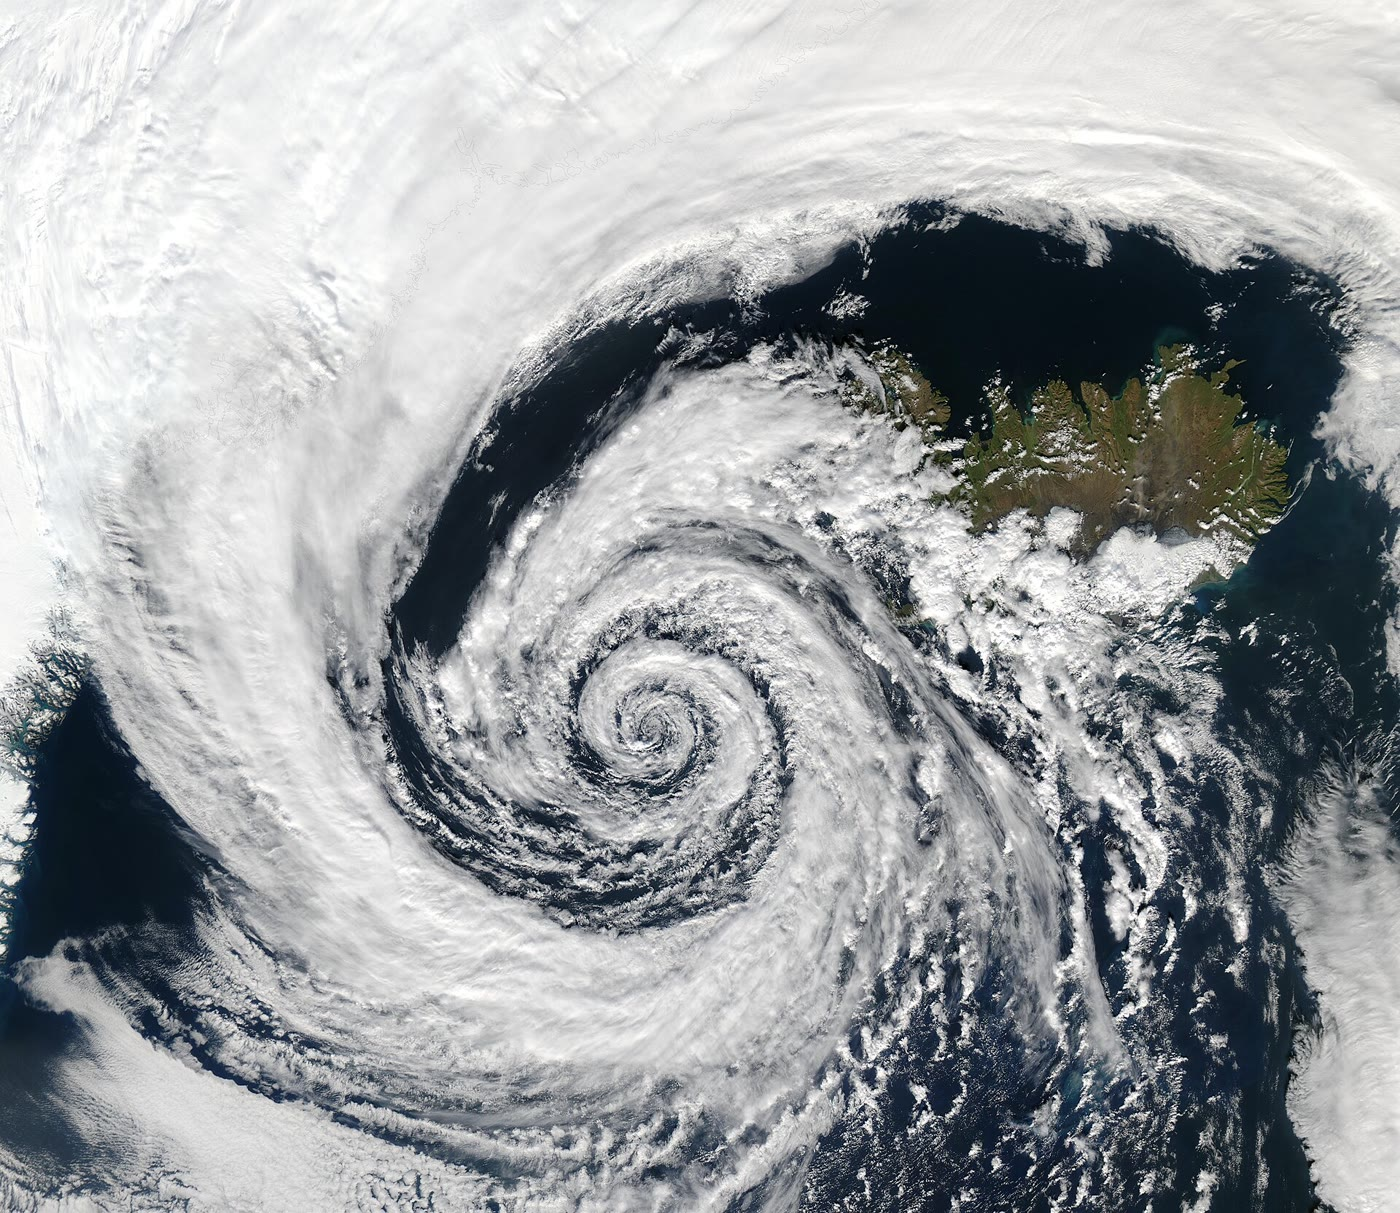
\includegraphics[width=\linewidth]{images/book1/g8-iceland-low.jpg}
\end{minipage}\hfill
\begin{minipage}[c]{0.6\linewidth}\raggedright
{\small Une \omterm{def:g8:fronts-and-weather-maps:depression}{dépression} au sud-ouest de l'Islande (l'île en haut à droite),
vue par le satellite Aqua de la NASA le 4~septembre 2003. Ses \omterm{def:g4:clouds-rain-snow:cloud}{nuages}
s'enroulent en spirale vers le centre, en tournant dans le sens inverse
des aiguilles d'une montre, comme dans toute \omterm{def:g8:fronts-and-weather-maps:depression}{dépression} de l'\omterm{def:g3:continents-and-oceans:equator}{hémisphère}
Nord. NASA/GSFC, MODIS Rapid Response Team, Jacques Descloitres (domaine
public, via Wikimedia Commons).}
\end{minipage}
% ledger: commons:iceland-low, bom:highs-lows
\label{fig:g8:fronts-and-weather-maps:iceland}
\end{omfigure}

\section{Isobares et cartes météorologiques}

Pour voir les \omterm{def:g8:fronts-and-weather-maps:depression}{dépressions} et les \omterm{def:g8:fronts-and-weather-maps:depression}{anticyclones}, les prévisionnistes
dessinent des \omterm{def:g2:drawing-to-map:map}{cartes} de la pression. Chaque station mesure sa pression et
la ramène au \omterm{def:g4:world-physical-map:altitude}{niveau de la mer}, pour qu'une station en \omterm{def:g1:landscapes-around-us:landform}{montagne} puisse être
comparée à une station sur la \omterm{def:g1:landscapes-around-us:water}{côte}. Puis on trace des lignes passant par
tous les lieux où la pression est la même.
% ledger: bom:isobars

\begin{definition}[Isobare]\label{def:g8:fronts-and-weather-maps:isobar}
Une \emph{isobare}\index{isobare} est une ligne qui, sur une \omterm{def:g2:drawing-to-map:map}{carte}, joint
les lieux où la pression au \omterm{def:g4:world-physical-map:altitude}{niveau de la mer} est la même. Les isobares
sont graduées en hectopascals et souvent tracées tous les \qty{4}{hPa}.
\end{definition}
% ledger: bom:isobars (the 4 hPa step is the one of this book's maps)

Autour d'une \omterm{def:g8:fronts-and-weather-maps:depression}{dépression}, les \omterm{def:g8:fronts-and-weather-maps:isobar}{isobares} forment des boucles fermées, avec la
pression la plus basse au centre, marqué D~; autour d'un \omterm{def:g8:fronts-and-weather-maps:depression}{anticyclone},
elles forment des boucles avec la pression la plus haute au centre, marqué
A. Là où les \omterm{def:g8:fronts-and-weather-maps:isobar}{isobares} sont serrées, la pression change vite d'un endroit à
l'autre, et le vent est fort~; là où elles sont écartées, le vent est
faible.
% ledger: bom:isobars

\begin{omfigure}
\begin{tikzpicture}
\begin{axis}[width=14cm, axis equal image, xmin=0, xmax=2400, ymin=0, ymax=1600,
  hide axis, clip=true, axis background/.style={fill=white}]
  \addplot[isobar] table {figdata/out/grade-8-weather_map-isobars.dat};
  \addplot[warm front] table {figdata/out/grade-8-weather_map-warm.dat};
  \addplot[cold front] table {figdata/out/grade-8-weather_map-cold.dat};
  \addplot[quiver={u=\thisrow{u}, v=\thisrow{v}}, -{Stealth[length=1.5mm]}, omMeth, line width=0.6pt]
    table[x=x, y=y] {figdata/out/grade-8-weather_map-winds.dat};
  \addplot[only marks, mark=none, nodes near coords, point meta=explicit symbolic,
    every node near coord/.style={anchor=center, font=\tiny, fill=white, inner sep=0.6pt}]
    table[x=x, y=y, meta=level] {figdata/out/grade-8-weather_map-labels.dat};
  \node[font=\Large\bfseries, omCold, fill=white, inner sep=1pt] at (axis cs:690,1010) {D};
  \node[font=\scriptsize, anchor=north, fill=white, inner sep=0.5pt] at (axis cs:690,968) {980};
  \node[font=\Large\bfseries, omWarm] at (axis cs:1950,520) {A};
  \node[font=\scriptsize, anchor=north] at (axis cs:1950,485) {1034};
  \addplot[only marks, mark=square*, mark size=2pt, black] table[x=x, y=y] {figdata/out/grade-8-weather_map-town.dat};
  \node[font=\footnotesize\bfseries, anchor=west, fill=white, inner sep=1pt] at (axis cs:870,380) {T};
  \fill[white] (axis cs:1930,1450) rectangle (axis cs:2290,1585);
  \draw[line width=1pt] (axis cs:1950,1480) -- (axis cs:2250,1480);
  \pgfplotsinvokeforeach{1950,2050,2150,2250}{\draw (axis cs:#1,1460) -- (axis cs:#1,1500);}
  \node[font=\scriptsize, anchor=south] at (axis cs:2100,1495) {300 km};
\end{axis}
\end{tikzpicture}

{\small Une \omterm{def:g2:drawing-to-map:map}{carte} \omterm{def:g1:watching-the-weather:weather}{météorologique} d'une journée imaginaire dans
l'\omterm{def:g3:continents-and-oceans:equator}{hémisphère} Nord, calculée à partir d'un modèle de la pression. \omterm{def:g8:fronts-and-weather-maps:isobar}{Isobares}
tous les \qty{4}{hPa}~; la \omterm{def:g8:fronts-and-weather-maps:depression}{dépression} D (\qty{980}{hPa}) porte un \omterm{def:g8:fronts-and-weather-maps:front}{front
chaud} (en rouge) et un \omterm{def:g8:fronts-and-weather-maps:front}{front froid} (en bleu)~; l'\omterm{def:g8:fronts-and-weather-maps:depression}{anticyclone} A
(\qty{1034}{hPa}) se trouve à l'est. Flèches vertes~: le vent, plus
longues là où il est plus fort. T~: la ville du problème.}
% ledger: bom:isobars, bom:highs-lows, mo:fronts (figdata/grade-8/weather_map.py)
\label{fig:g8:fronts-and-weather-maps:map}
\end{omfigure}

\begin{method}[Lire une carte météorologique]
\begin{enumerate}
  \item Trouve les centres~: D pour les \omterm{def:g8:fronts-and-weather-maps:depression}{dépressions}, A pour les
        \omterm{def:g8:fronts-and-weather-maps:depression}{anticyclones}, avec leurs pressions.
  \item Lis les \omterm{def:g8:fronts-and-weather-maps:isobar}{isobares}~: leurs valeurs montent vers A et descendent vers
        D. Des \omterm{def:g8:fronts-and-weather-maps:isobar}{isobares} serrées signifient un vent fort.
  \item Trouve la direction du vent~: dans l'\omterm{def:g3:continents-and-oceans:equator}{hémisphère} Nord, il souffle
        presque le long des \omterm{def:g8:fronts-and-weather-maps:isobar}{isobares}, avec les basses pressions à sa
        gauche, en tournant un peu vers la \omterm{def:g8:fronts-and-weather-maps:depression}{dépression}.
  \item Trouve les \omterm{def:g8:fronts-and-weather-maps:front}{fronts} et leur sens de déplacement (le côté de leurs
        symboles), puis l'air de chaque côté~: qu'est-ce qui arrive
        ensuite~?
\end{enumerate}
\end{method}
% ledger: bom:isobars, bom:highs-lows, mo:fronts

\begin{example}[Le temps dans la ville T]
Sur la \omterm{def:g2:drawing-to-map:map}{carte}, T se trouve au sud du \omterm{def:g8:fronts-and-weather-maps:front}{front chaud} et à l'est du \omterm{def:g8:fronts-and-weather-maps:front}{front
froid}~: dans l'air chaud, entre les deux \omterm{def:g8:fronts-and-weather-maps:front}{fronts}. Le \omterm{def:g8:fronts-and-weather-maps:front}{front chaud} est déjà
passé sur elle. Les \omterm{def:g8:fronts-and-weather-maps:isobar}{isobares} y vont du sud-ouest au nord-est, avec la
\omterm{def:g8:fronts-and-weather-maps:depression}{dépression} au nord-ouest~: le vent souffle du sud-ouest, chaud et humide.
Le \omterm{def:g8:fronts-and-weather-maps:front}{front froid} arrive de l'ouest. Ses triangles pointent vers l'est, vers
la ville~: d'ici quelques heures, il y aura une courte période de fortes
averses et de rafales, puis le vent tournera à l'ouest ou au nord-ouest,
l'air se rafraîchira et le ciel se dégagera.
\end{example}
% ledger: ucar:cold-front (figdata/grade-8/weather_map.py: wind at T from 227 degrees)

Un baromètre donne son propre avertissement, même sans \omterm{def:g2:drawing-to-map:map}{carte}. Suppose que
toute la \omterm{def:g2:drawing-to-map:map}{carte} ci-dessus se déplace vers l'est, sans changer, à
\qty{40}{km} à l'heure, et qu'un baromètre enregistreur se trouve à une
station S, à l'est des \omterm{def:g8:fronts-and-weather-maps:front}{fronts}. En deux jours et demi, il tracerait
l'enregistrement ci-dessous.

\begin{omfigure}
\begin{tikzpicture}
\begin{axis}[width=0.86\linewidth, height=5.4cm, xmin=0, xmax=60, ymin=980, ymax=1040,
  xtick={0,12,...,60}, ytick={980,990,...,1040},
  xlabel={heures depuis le début de l'enregistrement}, ylabel={pression (hPa)},
  axis x line=bottom, axis y line=left, axis line style={-},
  grid=major, grid style={black!10},
  tick label style={font=\scriptsize}, label style={font=\small}, clip=false]
  \draw[omWarm!80!black, dashed] (axis cs:26.28,980) -- (axis cs:26.28,1040);
  \draw[omCold!80!black, dashed] (axis cs:38.49,980) -- (axis cs:38.49,1040);
  \node[font=\scriptsize, omWarm!80!black, anchor=south, fill=white, inner sep=1pt] at (axis cs:26.28,1032) {front chaud};
  \node[font=\scriptsize, omCold!80!black, anchor=south, fill=white, inner sep=1pt] at (axis cs:38.49,1032) {front froid};
  \addplot[black!80, line width=1pt] table[x=hour, y=p_hPa] {figdata/out/grade-8-barogram-trace.dat};
  \node[font=\scriptsize, anchor=north west, align=left] at (axis cs:2,1028) {anticyclone~:\\temps stable};
  \node[font=\scriptsize, anchor=west] at (axis cs:39.5,986) {minimum};
\end{axis}
\end{tikzpicture}

{\small L'enregistrement d'un baromètre à la station S pendant que la \omterm{def:g2:drawing-to-map:map}{carte}
ci-dessus se déplace vers l'est à \qty{40}{km} à l'heure (une situation
inventée, calculée à partir du champ de pression de la \omterm{def:g2:drawing-to-map:map}{carte}). En
tirets~: le passage du \omterm{def:g8:fronts-and-weather-maps:front}{front chaud} et du \omterm{def:g8:fronts-and-weather-maps:front}{front froid} à la station.}
% ledger: (invented region: weather situation of figdata/grade-8/weather_map.py, record from figdata/grade-8/barogram.py)
\end{omfigure}

\begin{example}[Lire l'enregistrement d'un baromètre]\label{ex:g8:fronts-and-weather-maps:barogram}
Pendant les 8~premières heures, la pression monte jusque vers
\qty{1031}{hPa}~: l'\omterm{def:g8:fronts-and-weather-maps:depression}{anticyclone} passe sur S, avec un temps stable. Puis
elle baisse pendant 30~heures, d'environ \qty{45}{hPa}~: la \omterm{def:g8:fronts-and-weather-maps:depression}{dépression}
arrive. Elle baisse le plus vite quelques heures avant le passage du \omterm{def:g8:fronts-and-weather-maps:front}{front
chaud}, plus lentement dans l'air chaud qui le suit, et atteint son
minimum, environ \qty{986}{hPa}, juste au passage du \omterm{def:g8:fronts-and-weather-maps:front}{front froid}. Puis
elle remonte~: la \omterm{def:g8:fronts-and-weather-maps:depression}{dépression} s'éloigne, et l'air plus frais et plus clair
qui suit le \omterm{def:g8:fronts-and-weather-maps:front}{front froid} arrive.
% ledger: (invented region: figdata/grade-8/barogram.py), bom:highs-lows
\end{example}

\section{Comment se fait une prévision}

\begin{definition}[Prévision météorologique]\label{def:g8:fronts-and-weather-maps:forecast}
Une \emph{prévision météorologique}\index{prevision meteorologique@prévision météorologique}
est l'annonce du temps attendu en un lieu pour les heures ou les jours
à venir, établie à partir d'observations de l'atmosphère et des lois de la
physique.
\end{definition}
% ledger: mo:how-forecasts

Une prévision se fait en trois étapes. D'abord, les services
\omterm{def:g1:watching-the-weather:weather}{météorologiques} du monde entier font chaque jour des millions
d'observations~: température, \omterm{def:g4:clouds-rain-snow:precipitation}{précipitations}, pression, vent et humidité,
mesurés dans des stations au sol, en \omterm{def:g2:water-on-earth:ocean}{mer}, par des ballons-sondes, par des
radars et depuis des satellites. Ensuite, ces observations sont fournies à
des modèles informatiques~: des ordinateurs très puissants calculent, pas à
pas, comment l'atmosphère va évoluer à partir de son état présent. Enfin,
les prévisionnistes lisent les résultats, les comparent à ce qu'ils savent
de leur région, et rédigent la prévision.
% ledger: mo:how-forecasts

\begin{history}[La première prévision publique]
En 1854, un officier de marine, Robert FitzRoy, fut placé à la tête d'un
nouveau bureau \omterm{def:g1:watching-the-weather:weather}{météorologique} à Londres. Chaque matin à 9~h, des stations
réparties le long des \omterm{def:g1:landscapes-around-us:water}{côtes} mesuraient le temps et envoyaient leurs
relevés à Londres par le télégraphe, l'invention la plus récente de
l'époque. En 1859, une terrible \omterm{def:g5:natural-hazards:storm}{tempête}, la \omterm{def:g5:natural-hazards:storm}{tempête} du
\emph{Royal Charter}, coula de nombreux navires~; FitzRoy créa alors un
service d'avis de \omterm{def:g5:natural-hazards:storm}{tempête} pour les marins, qui commença en février 1861.
Le 1\textsuperscript{er}~août 1861, il alla plus loin et publia la
première \omterm{def:g8:fronts-and-weather-maps:forecast}{prévision météorologique} publique dans un journal,
\emph{The Times}. Ses prévisions portaient sur un ou deux jours et
restaient très générales~; elles furent le début des prévisions que nous
lisons aujourd'hui.
\end{history}
% ledger: mo:fitzroy

Les prévisions se sont beaucoup améliorées. Au cours des dernières
décennies, les prévisionnistes ont gagné environ un jour de bonne
prévision tous les dix ans~: une prévision à quatre jours est aujourd'hui
aussi bonne qu'une prévision à un jour il y a trente ans. Mais plus une
prévision regarde loin, moins elle est sûre, parce que de petites erreurs
dans les observations de départ grandissent à mesure que l'ordinateur
avance dans le temps.
% ledger: bauer:day-per-decade, mo:accuracy

\begin{inthefield}[Regarder un front arriver]
Un jour où la prévision annonce un \omterm{def:g8:fronts-and-weather-maps:front}{front}, regarde le ciel toutes les
quelques heures et note l'heure, les \omterm{def:g4:clouds-rain-snow:cloud}{nuages}, le vent et la température.
Avant un \omterm{def:g8:fronts-and-weather-maps:front}{front chaud}, de hautes traînées de \omterm{def:g4:clouds-rain-snow:cloud-families}{cirrus} arrivent-elles en
premier~? Quand un \omterm{def:g8:fronts-and-weather-maps:front}{front froid} passe, la température baisse-t-elle, et le
vent change-t-il~? Compare tes notes avec la \omterm{def:g2:drawing-to-map:map}{carte} \omterm{def:g1:watching-the-weather:weather}{météorologique} du jour.
\end{inthefield}

\section{Exercices}

\begin{exercise}[$\star$]\label{exo:g8:fronts-and-weather-maps:1}
Donne le sens de chaque paire de lettres et dis si la \omterm{def:g8:fronts-and-weather-maps:air-mass}{masse d'air} est
chaude ou froide, humide ou sèche~: (a) mT~; (b) cP~; (c) cT~; (d) mP.
\end{exercise}

\begin{exercise}[$\star$]\label{exo:g8:fronts-and-weather-maps:2}
Associe chaque signe d'une \omterm{def:g2:drawing-to-map:map}{carte} \omterm{def:g1:watching-the-weather:weather}{météorologique} à son sens~: une ligne
bleue à triangles~; une ligne rouge à demi-cercles~; une ligne qui joint
des lieux de même pression~; la lettre A~; la lettre D.
\end{exercise}

\begin{exercise}[$\star$]\label{exo:g8:fronts-and-weather-maps:3}
Vrai ou faux~? Corrige les phrases fausses. (a) Les \omterm{def:g8:fronts-and-weather-maps:depression}{anticyclones} apportent
en général un temps stable. (b) Les \omterm{def:g4:clouds-rain-snow:cloud}{nuages} d'un \omterm{def:g8:fronts-and-weather-maps:front}{front chaud} arrivent après
le \omterm{def:g8:fronts-and-weather-maps:front}{front}. (c) Des \omterm{def:g8:fronts-and-weather-maps:isobar}{isobares} serrées signifient un vent faible. (d) L'air
froid est plus dense que l'air chaud.
\end{exercise}

\begin{exercise}[$\star$]\label{exo:g8:fronts-and-weather-maps:4}
Sur la \omterm{def:g2:drawing-to-map:map}{carte} \omterm{def:g1:watching-the-weather:weather}{météorologique} de ce chapitre~: (a) quelle est la pression au
centre de la \omterm{def:g8:fronts-and-weather-maps:depression}{dépression}~? (b) Au centre de l'\omterm{def:g8:fronts-and-weather-maps:depression}{anticyclone}~? (c) Combien
d'hectopascals séparent deux \omterm{def:g8:fronts-and-weather-maps:isobar}{isobares} voisines~? (d) De combien
d'hectopascals la pression diffère-t-elle entre les deux centres~?
\end{exercise}

\begin{exercise}[$\star\star$]\label{exo:g8:fronts-and-weather-maps:5}
Range ces événements dans l'ordre où ils se produisent quand un \omterm{def:g8:fronts-and-weather-maps:front}{front
chaud} approche puis passe~: une \omterm{def:g4:clouds-rain-snow:precipitation}{pluie} continue~; de fines traînées de
\omterm{def:g4:clouds-rain-snow:cloud-families}{cirrus}~; un voile gris d'altostratus~; un air plus chaud et plus humide~;
les \omterm{def:g4:clouds-rain-snow:cloud}{nuages} qui descendent et s'épaississent.
\end{exercise}

\begin{exercise}[$\star\star$]\label{exo:g8:fronts-and-weather-maps:6}
Explique pourquoi les \omterm{def:g4:clouds-rain-snow:cloud}{nuages} d'un \omterm{def:g8:fronts-and-weather-maps:front}{front froid} s'élèvent comme des tours,
alors que ceux d'un \omterm{def:g8:fronts-and-weather-maps:front}{front chaud} s'étalent en couches. Utilise les mots
\emph{coin}, \emph{brusquement}, \emph{pente douce}.
\end{exercise}

\begin{exercise}[$\star\star$]\label{exo:g8:fronts-and-weather-maps:7}
Sur la \omterm{def:g2:drawing-to-map:map}{carte} \omterm{def:g1:watching-the-weather:weather}{météorologique}~: (a) où le vent est-il le plus fort, près de D
ou près de A~? Comment le sais-tu~? (b) Au nord de D, de quelle direction
souffle le vent~? (c) Au sud de A~? (d) Le vent tourne-t-il autour de D
dans le sens des aiguilles d'une montre ou dans le sens inverse~?
\end{exercise}

\begin{exercise}[$\star\star$]\label{exo:g8:fronts-and-weather-maps:8}
Un baromètre, dans une ville, indique \qty{1016}{hPa} à 6~h,
\qty{1009}{hPa} à 12~h et \qty{1003}{hPa} à 18~h. (a) De combien la
pression baisse-t-elle en 12~heures~? (b) Qu'est-ce qui arrive vers la
ville, une \omterm{def:g8:fronts-and-weather-maps:depression}{dépression} ou un \omterm{def:g8:fronts-and-weather-maps:depression}{anticyclone}~? (c) Quel temps la ville
peut-elle attendre~?
\end{exercise}

\begin{exercise}[$\star\star$]\label{exo:g8:fronts-and-weather-maps:9}
De l'air qui est resté une semaine au-dessus du Sahara se déplace vers le
nord au-dessus de la \omterm{def:g2:water-on-earth:ocean}{mer} Méditerranée. (a) Désigne cette \omterm{def:g8:fronts-and-weather-maps:air-mass}{masse d'air} par
ses deux lettres. (b) Est-elle chaude ou froide, humide ou sèche, au
départ~? (c) Qu'est-ce qui pourrait changer dans son caractère pendant
qu'elle traverse la \omterm{def:g2:water-on-earth:ocean}{mer}~?
\end{exercise}

\begin{exercise}[$\star\star$]\label{exo:g8:fronts-and-weather-maps:10}
Une prévision à quatre jours est aujourd'hui aussi bonne qu'une prévision
à un jour il y a trente ans. (a) Combien de jours de bonne prévision
ont été gagnés en trente ans~? (b) Combien cela fait-il pour dix ans~?
(c) Si le même progrès continuait, dans combien d'années une prévision à
cinq jours serait-elle aussi bonne que la prévision à un jour
d'aujourd'hui~?
\end{exercise}

\begin{exercise}[$\star\star\star$]\label{exo:g8:fronts-and-weather-maps:11}
Sur la \omterm{def:g2:drawing-to-map:map}{carte} \omterm{def:g1:watching-the-weather:weather}{météorologique}, utilise l'\omterm{def:g2:drawing-to-map:scale}{échelle} graphique. (a) Environ
combien de kilomètres séparent le centre D du centre A~? (b) Près de D,
deux \omterm{def:g8:fronts-and-weather-maps:isobar}{isobares} voisines sont à environ \qty{80}{km} l'une de l'autre. De
combien d'hectopascals la pression change-t-elle sur \qty{100}{km} à cet
endroit~? (c) Près de A, deux \omterm{def:g8:fronts-and-weather-maps:isobar}{isobares} voisines sont à environ
\qty{140}{km} l'une de l'autre. Même question. (d) Où le vent est-il le
plus fort~? Les flèches de la \omterm{def:g2:drawing-to-map:map}{carte} sont-elles d'accord~?
\end{exercise}

\begin{exercise}[$\star\star\star$]\label{exo:g8:fronts-and-weather-maps:12}
Un \omterm{def:g8:fronts-and-weather-maps:front}{front froid} se trouve à \qty{300}{km} à l'ouest d'une ville et avance
vers l'est à \qty{50}{km} par heure~; un \omterm{def:g8:fronts-and-weather-maps:front}{front chaud} se trouve à
\qty{200}{km} à l'ouest d'une autre ville et avance deux fois moins vite.
(a) Quel \omterm{def:g8:fronts-and-weather-maps:front}{front} atteint sa ville le premier, et combien d'heures plus
tôt~? (b) Décris le temps que verra chaque ville au passage de son \omterm{def:g8:fronts-and-weather-maps:front}{front}.
(c) Quelle ville sera la plus chaude une fois son \omterm{def:g8:fronts-and-weather-maps:front}{front} passé~?
\end{exercise}

\section{Problème~: Le match sera-t-il annulé à cause de la pluie~?}

\begin{problem}[{Problème du week-end --- un match de football est prévu à 15~h
dans la ville T de la carte météorologique~; le front froid arrive~: sa
vitesse est mesurée sur deux cartes et l'on prévoit l'heure à laquelle il
atteint la ville}]
\label{pb:g8:fronts-and-weather-maps:1}
% ledger: ucar:cold-front (figdata/grade-8/weather_map.py; the front's speed and the length of the showers are exercise data)
À 9~h, une jeune prévisionniste regarde la \omterm{def:g2:drawing-to-map:map}{carte} \omterm{def:g1:watching-the-weather:weather}{météorologique} de ce
chapitre, puis la \omterm{def:g2:drawing-to-map:map}{carte} ci-dessous~: elle montre le \omterm{def:g8:fronts-and-weather-maps:front}{front froid} près de la
ville à 6~h et à 9~h, sur un quadrillage de carreaux de \qty{20}{km}.

\begin{center}
\begin{tikzpicture}
\begin{axis}[width=11cm, axis equal image, xmin=0, xmax=600, ymin=0, ymax=400,
  xtick={0,100,...,600}, ytick={0,100,...,400}, minor tick num=4,
  grid=both, minor grid style={black!10}, major grid style={black!25},
  tick label style={font=\scriptsize}, xlabel={distance vers l'est (km)}, ylabel={distance vers le nord (km)},
  label style={font=\small}]
  \addplot[cold front, densely dashed, opacity=0.55] table[x expr=\thisrow{x}-363.2, y expr=\thisrow{y}-180] {figdata/out/grade-8-weather_map-seq-06.dat};
  \addplot[cold front] table[x expr=\thisrow{x}-363.2, y expr=\thisrow{y}-180] {figdata/out/grade-8-weather_map-seq-09.dat};
  \addplot[only marks, mark=square*, mark size=2.2pt, black] table[x expr=\thisrow{x}-363.2, y expr=\thisrow{y}-180] {figdata/out/grade-8-weather_map-town.dat};
  \node[font=\footnotesize\bfseries, anchor=south west, fill=white, inner sep=1pt] at (axis cs:485,205) {T};
  \node[font=\scriptsize, fill=white, inner sep=1pt] at (axis cs:140,360) {6~h};
  \node[font=\scriptsize, fill=white, inner sep=1pt] at (axis cs:262,360) {9~h};
\end{axis}
\end{tikzpicture}
\end{center}

\noindent\textbf{Partie I --- Lire la carte.}\par\nopagebreak
\begin{enumerate}[beginpenalty=10000]
  \item Sur la \omterm{def:g2:drawing-to-map:map}{carte} \omterm{def:g1:watching-the-weather:weather}{météorologique} du chapitre, la ville est-elle dans
        l'air chaud ou dans l'air froid~? Quel \omterm{def:g8:fronts-and-weather-maps:front}{front} est déjà passé sur
        elle~?
  \item De quelle direction souffle le vent dans la ville~?
  \item Dans quel sens avance le \omterm{def:g8:fronts-and-weather-maps:front}{front froid}~? Comment le vois-tu à ses
        symboles~?
  \item Quel temps le \omterm{def:g8:fronts-and-weather-maps:front}{front froid} apportera-t-il à son passage~?
\end{enumerate}

\noindent\textbf{Partie II --- La vitesse du front.}\par\nopagebreak
\begin{enumerate}[resume, beginpenalty=10000]
  \item Sur la \omterm{def:g2:drawing-to-map:map}{carte} ci-dessus, à la hauteur de la ville, à quelle
        distance vers l'est se trouve le \omterm{def:g8:fronts-and-weather-maps:front}{front} à 6~h~? À 9~h~?
  \item De combien de kilomètres le \omterm{def:g8:fronts-and-weather-maps:front}{front} s'est-il déplacé en ces trois
        heures~?
  \item Quelle est sa vitesse, en kilomètres par heure~?
  \item À 9~h, combien de kilomètres séparent le \omterm{def:g8:fronts-and-weather-maps:front}{front} de la ville~?
\end{enumerate}

\noindent\textbf{Partie III --- La prévision.}\par\nopagebreak
\begin{enumerate}[resume, beginpenalty=10000]
  \item Si le \omterm{def:g8:fronts-and-weather-maps:front}{front} garde la même vitesse, combien d'heures lui faudra-t-il
        pour atteindre la ville~?
  \item À quelle heure atteindra-t-il la ville~?
  \item Suppose que les fortes averses durent environ une heure après le
        passage du \omterm{def:g8:fronts-and-weather-maps:front}{front}. Pleuvra-t-il encore à 15~h~?
  \item Le \omterm{def:g8:fronts-and-weather-maps:front}{front} pourrait ralentir à \qty{30}{km} par heure. Quand
        atteindrait-il alors la ville~? Écris la prévision pour le match en
        une ou deux phrases, en donnant les deux heures possibles.
\end{enumerate}
\end{problem}
